\chapter{Sea: A lightweight data-management library for Big Data scientific computing}\label{chapter:sea-comp}
% remove neuroimaging and replace with scientific computing  add user-space,
% switch HPC to computing clusters

Val\'erie Hayot-Sasson and Tristan Glatard \\
\begingroup \footnotesize Department of Computer Science and Software
Engineering, Concordia University, Montreal, Canada \\
\endgroup 
\vspace{5pt} \\
Manuscript in preparation. \\

\section{Abstract}

The recent influx of scientific computing datasets have shifted scientific computing
from compute intensive to data intensive. Whereas many Big Data Frameworks exist that
minimize the cost of data transfers, few scientific applications adopt data-management
strategies as the effort required to update the existing applications is significant.

We developed Sea as a means to enable data-management strategies for scientific applications
executing on HPC clusters
without needing to update the underlying applications. Sea leverages GNU libc interception to intercept
POSIX-compliant filesystem calls made by the applications. We design and performance model and
evaluated the performance of Sea on a synthetic data-intensive application processing a representative 
neuroimaging dataset (the Big Brain). Our results demonstrate that Sea significantly improves 
performance, up to a factor of 3$\times$. 

\section{Introduction}\label{sec:introduction}
Efficient data-management
strategies have become essential in minimizing the costs of processing Big Data.
Such strategies include data locality and in-memory computing, which minimize
transfers by ensuring compute occurs where the data is located and maintain data
in the fastest available storage (i.e. memory). Big Data frameworks, such as
MapReduce~\cite{dean2008mapreduce}, Apache Spark~\cite{zaharia2016apache} and
Dask~\cite{rocklin2015dask}, provide such data management mechanisms by default.

Until the recent surge in publicly available scientific data, scientific
workflows had been regarded as compute intensive. As a result, standardized
scientific tools typically lack these data-management mechanisms. The sheer
effort required to update the applications to leverage Big Data frameworks
(e.g. changing framework, programming language, training staff) can be a
significant deterrent. Furthermore, Big Data frameworks still require
significant work to be well adapted for the processing of different scientific
data, such as imaging data~\cite{mehta2017comparative}.



% add speedup results

% Many scientific applications, such as those found in geography and
% neuroscience, perform image processing. However,  BigData frameworks were
% originally developed for text-processing and have only recently incorporated
% components that could facilitate the processing of images. The fundamental
% differences between these two data formats make leveraging BigData frameworks
% for scientific image processing non-trivial, even considering recent advances.
% 

%Scientific applications are usually composed of numerous well-established
%command-line tools. These tools may have been developed at a time when
%processing would have been compute intensive, thus do not incorporate data
%management strategies. While newer applications that leverage such tools may be
%written using Big Data frameworks, such frameworks are not designed to transfer
%data in-memory to command-line applications, making it difficult to incorporate
%these tools without additional overhead.

Our goal is to provide data management strategies to scientific tools. We focus
on well-established scientific applications that operate as command-line tools.
These applications are written in a variety of different programming languages
and communicate data between tasks via a POSIX-compliant shared file system.

Scientific tools are typically platform agnostic with the exception that the
filesystem must be POSIX-compliant. That is, they can run on local workstations,
high performance computing (HPC) clusters and cloud infrastructure, with the
exception that they cannot communicate with a cloud-based storage natively. We
focus our efforts on HPC clusters as they are widely used in scientific
computing and are currently used for the processing of scientific Big Data.

% Although various infrastructures are available to researchers, such as local
% workstations, the cloud (AWS, ..etc) and High Performance Computing (HPC)
% clusters, researchers commonly rely on HPC clusters due to their low cost and
% available resources. Such clusters typically rely on a network-based parallel
% file system, such as Lustre, Ceph and GlusterFS. Since data storage and
% compute are maintained as separate entities on HPC clusters, processing
% BigData workflows on them may be particularly costly, particularly when no
% BigData framework is applied. Furthermore, while it is possible to execute
% workloads using BigData frameworks on HPC, these frameworks are typically
% incompatible with the native resource managers (e.g. SLURM, PBS), and
% therefore, and overlay cluster must be used.

In this paper we introduce Sea, a user-space hierarchical file system for
scientific workloads. The aim of Sea is to bring Big Data performance to
scientific workloads through the incorporation of data locality and in-memory
computing. Unlike Big Data frameworks, Sea can be utilized alongside existing
workloads without the need to entirely reinstrument the existing workload.
Furthermore, as it executes entirely in userspace, it does not require elevated
privileges to be installed and executed.

This paper makes the following contributions:
\begin{itemize}
    \item Introduces a library, Sea, that generates an on-the-fly user-space
    hierarchical filesystem
    \item Develops a model to describe the performance bound that can be
    obtained through the use of Sea
    \item Evaluates the tool using a synthetic Big Data workload on a real
    neuroimaging dataset
\end{itemize}

%multiple disk support pipeline agnostic and pipeline access patterns don't
% leverage workflows leverage existing filesystems replace storage devices with
% storage location. use applications memory management paragraph: PAGE CACHE
% shared filesystems are slow and metadata management can be slow




% add need for userspace / intelligent pipeline flushing there is no one-size
% fits all with data intensive applications due to io patterns, so we decided
% with userspace.


% add related work section
\section{Related Work}
\subsection{HPC Infrastructure}
      The general structure of HPC clusters may complicate the deployment of Big
      Data frameworks. Typical HPC clusters consist of distinct storage and
      compute nodes. While the compute nodes may also have local storage, there
      is no distributed file system like the Hadoop Distributed File System
      (HDFS)~\cite{shvachko2010hadoop} or Alluxio~\cite{alluxio} to facilitate
      data locality. Furthermore, access to these compute nodes is temporary,
      with allocation duration enforced by a batch scheduler. Therefore, any
      data written to a compute node is inaccessible after the allocation is
      terminated.

      The storage layer found on HPC clusters consists of a high-performance
      parallel file system (PFS) (e.g Lustre~\cite{lustre}). These file systems
      are shared amongst all compute nodes within a cluster, typically connected
      to each node via high-performance network interconnect such as
      InfiniBand~\cite{infiniband}. I/O overheads to shared PFS can be incurred
      in many places, from the shared network, to the bandwidth of the storage
      disks.  With Lustre specifically, there are many data nodes, known as
      Object Storage Servers (OSS) which contain several storage devices, known
      as Object Storage Targets (OST). All file metadata is maintained within a
      separate node known as the Metadata Server (MDS) and stored within a
      device referred to as the Metadata Target (MDT). Although data transfers
      can be communicated directly to the corresponding OST, the clients need to
      first communicate with the MDS to determine which OST to communicate with.
      This can result in data transfer overheads, particularly when making
      numerous requests to the metadata server.
      
      
      HPC clusters may provide a faster additional storage layer, known as a
      Burst Buffer, aimed at improving I/O performance. A Burst Buffer typically
      consists of fast storage (SSD and memory) and can be local to the compute
      node or as a dedicated I/O node. It was introduced as a response to offset
      the impacts of large-scale application checkpointing on the PFS. The
      application would write a checkpoint to the Burst Buffer and resume
      processing, while the checkpoint would be asynchronously flushed to the
      PFS. 


\subsection{Big Data Frameworks and File systems}

      Strategies to facilitate the processing of such large datasets is
      required. In text-based processing, frameworks such as
      MapReduce~\cite{dean2008mapreduce} and Apache Spark~\cite{zaharia2016apache} have implemented
      and popularized strategies to minimize the need for data transfers during
      processing. These strategies are known as data locality and in-memory
      computing.

      Data locality is the process by which compute tasks are scheduled nearest
      to where the data is located. Traditionally, storage and compute were kept
      separate, having to transfer data over the network to compute. Rather than
      having to transfer large amounts of data over the network to the compute
      tasks, which could incur significant overheads, Big Data frameworks ensure
      that data is stored directly on the compute nodes. When a compute task
      requires access to specific data, the scheduler sends the task to the
      nearest available node to the data, thereby minimizing any cost of
      network-related data transfers. This strategy is not only used by Big Data
      Frameworks such as Hadoop MapReduce, Apache Spark, and Dask~\cite{rocklin2015dask},
      but also enabled by file systems such as HDFS and Alluxio.



\subsection{The Linux page cache}
 While scientific applications uncommonly use Big Data frameworks and must
      perform large over-the-network data transfers, they may still benefit from
      in-memory computing and data locality through the Linux Page
      Cache~\cite{pagecache}. Similarly to other filesystems, Lustre leverages
      the client node page cache to reduce I/O overheads. System memory is
      composed of two components: 1) anonymous memory and 2) page cache.
      Anonymous memory consists of all application-related objects, whereas page
      cache consists of recently accessed file data. When a file is read, that
      file is loaded up into the page cache to be flagged for eviction based on
      a least recently used (LRU) policy. That means subsequent accesses to that
      data may be done entirely in memory so long as that data has not already
      been evicted. Similarly, for writes to a file system with writeback cache
      enable, the file will be written to memory completing the write operation
      once the file has been written entirely to memory. That file will then be
      flushed asynchronously to the appropriate storage device. As system memory
      may get overloaded with too many write requests, there is a limit to the
      amount of written data that can exist in memory, known as the
      \texttt{dirty\_ratio}. Furthermore, applications producing too many write
      requests may be throttled by the system.

\subsection{File System implementations}
      Due to the architecture of conventional HPC clusters, network-based
      parallel files systems are favoured over Big Data distributed filesystems.
      Such filesystems require super-user access, preventing users from
      deploying their own own on-the-fly cluster. While HDFS can be loaded in
      user-space by mounting its File System in Userspace (FUSE) implementation,
      FUSE-based filesystems can perform significantly worse than desired,
      depending on the application~\cite{tofuse}. Even with a user-space version
      of HDFS, there would be no mechanism to transfer all the data back to the
      parallel filesystem to be accessible post resource requests. Furthermore,
      such filesystems are not POSIX-compliant, which would be required for
      scientific computing applications.
      
      There are, however, BigData filesystems, such as XtreemFS~\cite{xtreemfs}
      that exist entirely within user space, are POSIX-compliant, and can use
      alternative methods to FUSE to function. XtreemFS uses 
      the LD\_PRELOAD trick to intercept filesystem calls
      made to the GNU libc library. There are limitations to using libc
      interception. For instance, the application must be dynamically linked and
      make libc calls. However, statically-linked applications are uncommon and
      applications interacting with POSIX-compliant file systems on Linux
      machines, the predominant OS of HPC clusters, will make libc calls.
      Nevertheless, there are alternatives to libc intercept that can bypass the
      aforementioned issues, such as system call interception, but they result
      in greater overheads~\cite{quinson}.

      Characteristics that make XtreemFS unlikely to be deployed on-the-fly
      include complex filesytem deployment and configuration properties. It also
      does not provide a simple way to leverage different classes of storage
      devices, nor ensure that required data will be copied to the cluster's
      parallel file system.

      BurstFS~\cite{burstfs} and GekkoFS~\cite{gekkofs} are two user-space
      filesystems that are specifically designed for Burst Buffers. That is,
      both of these filesystems exist only during the time-window in which the
      resources are allocated. Furthermore, they both exist entirely within
      user-space using libc interception. While these implementations simplify
      usage of burst buffers for users, their configuration would be out of the
      scope of a typical HPC user and thus require sysadmin intervention.
      %include triple-H
%\subsubsection{Kernel-space file systems} add comments in methods
%\subsubsection{Unionfs} \subsubsection{FUSE} add number w/o plot
%\subsubsection{System call interception with ptrace}
%\subsubsection{LD\_PRELOAD} xtreemfs/xtreemos

\section{Materials and Methods}

\subsection{Sea design and implementation}

Sea\footnote{\url{https://github.com/valhayot/sea}} is an open-source user-space data-management C++ library for applications running on HPC
systems. Its main aim is to reduce application data transfer costs by leveraging
node-local storage. Sea redirects files accessed from a user-specified mount
point to the appropriate storage devices using libc interception. Within an
intercepted call the file will be written to or read from the fastest storage
device available. 


At minimum, Sea requires the user to specify at least two storage devices, a
fast temporary one and a slower long-term storage one. This could be RAM and SSD
if working on a single node, or a compute-local SSD and a shared parallel file
system, in the case of an HPC cluster. Ideally, a user will provide a multitude
of short-term storage devices to improve Sea's efficacy. Furthermore, to
maximize usage of the fastest available storage devices, Sea will allow the user
to outline which files can be removed from short-term storage in addition to
which files need to be materialized onto long-term storage. Eviction of files is
important as this will allow Sea to maximize usage of short-term storage.


Sea was meant as a data-management service to be employed at the discretion of
the users on scientific applications. When coming up with the idea for Sea, we
observed the design differences between Big Data and scientific, specifically
neuroimaging, frameworks and applications. Scientific frameworks tend to favour
ease-of-use, reproducibility, portability and parallelism over minimizing data
transfers. It was important for us to ensure that Sea would preserve the design
decisions of the underlying tools. Sea achieves this by having few dependencies,
is lightweight, and requires minimal configuration.


In this subsection, we will discuss and outline the various design and
implementation details made. Furthermore, we will go into detail into the
functionality of Sea.

\subsubsection{Requirements and assumptions}

Sea is primarily designed to work with workloads that generate large amounts of
intermediate data. Since data must be read from the slower storage device and
final output data most likely would have to be written to the same device, the
use of Sea with workloads that do not produce intermediate data would result in
limited speedup and may even introduce some overheads. 

Sea provides two main modes performance bounds based on flushing specification:
In-memory computing and flush-all. In-memory computing is achieved when
intermediate need not be materialized to long-term storage (i.e. no flushing).
With Sea in-memory, we can expect speedups comparable to Big Data frameworks.

As the name implies, Sea flush-all is achieved when all data must be
materialized to long-term storage (i.e. flush everything). This can be coupled
with eviction to limit the amount of data that will be written to slower, but
larger local storage devices. While this option will have overheads, due to the
need to flush all application data, performance can be improved when data
transfers and compute time are similar. 

% Occasionally, it is desired to materialize even intermediate data to long-term
% storage devices, for potential future use. The performance gain from using Sea
% in these scenarios, however, is largely bounded by data size. In the instances
% where the workloads is more compute intensive, we can gain speedup by masking
% all or part of the I/O through long-term storage by executing the flush during
% a compute task. In data-intensive scenarios, the opposite can be seen: compute
% time can be masked by I/O (add figure + model). Despite the performance gain
% being limited in such a scenario, a performance gain can still be observed
% through the use of Sea.

One important assumption that must be made is that the amount of data produced
by the workload far exceeds the amount of page cache space available and
utilized by the different filesystems. In the case where all workload data can
fit into page cache memory, the benefit of Sea may be greatly diminished if not
negligible.

Naturally, the amount of data written may not fit entirely into a single local
storage location. Currently, the user cannot specify the maximum amount of space
to use in a given mountpoint explicitly. Sea queries all the available
filesystem directly to determine the amount of available space. It relies on
user-specified information on the maximum file size produced by the pipeline and
the number of concurrent pipeline parallel threads to determine if there is
sufficient space to write to the file system without issue. While it prevent
overheads due to locking, it makes the assumption that the user is alone writing
to the storage device. The user can reduce the amount of local storage space
used by increasing the maximum file size of the application.

%\todo{depending on the version of libc, the application static/dynamic linking,
%version of the function}


\subsubsection{Benefits}
Sea removes the need to implement the logic to redirect data to the appropriate
storage locations. Furthermore, it implements logic to ensure that files are
written to the best possible location at any given time. It is both pipeline and
infrastructure agnostic.

As it executes in user-space, root permissions are not required, enabling users
to use Sea on most Linux-based systems available to them. This differs from Big
Data filesystems which may require elevated permissions to install. The overhead
of intercepting libc calls is minimal, and negligible compared to system call
interception and file systems such as FUSE.

Unlike Big Data frameworks, Sea does not require reinstrumentation of the
existing pipelines, allowing users to gain an instant performance boost.

\subsubsection{Libc interception}

Libc interception is achieved by writing wrappers to existing libc functions.
Most importantly, every libc function accepting a file path needs to be wrapped.
The wrappers take any input filepath that is located within the
user-provided Sea mountpoint and convert it a filepath pointing to the best
available storage device.

Sea does not currently support the partitioning of files across multiple
devices. Since it cannot predict the size of the outputs to ensure the existence
of sufficient space on storage devices, the user must provide within the Sea
configuration file the maximum file size produced by the workflow. Together with
the specified amount of parallel processes, Sea calculates the minimum space
required on a storage device to write the file to it.
%\todo{should include an equation here}
Sea will then go through the hierarchy of available storage devices an select
the fastest storage device with sufficient available space. While this process
may result in not utilizing all available space in fast storage devices, it will
still allow users to gain a performance speedup on the pipeline given that the
number of threads multiplied by the file size does not exceed storage space.

\subsubsection{Installation and execution}
Users wanting to use Sea will need to compile the library via GCC (C++11) and
Make, or use one of our pre-made containers available on
GitHub\footnote{\url{https://github.com/ValHayot?tab=packages&repo_name=Sea}}.
If compiling, users will need to ensure that the dependencies,
\href{https://github.com/ndevilla/iniparser}{libiniparser} and libmagic, are
met.

Once the library is compiled, users will need to select a directory to be set as
the SEA\_HOME environment variable. This directory will contain the Sea
configuration file (\texttt{sea.ini}) and three files consisting of data to be
prefetched to caches (\texttt{.sea\_prefetchlist}), flushed from cache
(\texttt{.sea\_flushlist}) and evicted from cache (\texttt{.sea\_evictlist}).

Whereas prefetching, flushing and eviction files are all optional, the
configuration file is not. When running Sea for the first time, if the
configuration file is missing, Sea will not be launched and an example
configuration file will be generated. Within this configuration file, users will
have to specify the available storage locations (i.e. local storage and PFS) according to 
the preferred hierarchy, as
well as the Sea prefix to use (called the ``mountpoint''), log level and log
file path and maximum file size and number of parallel processes.

With a properly set SEA\_HOME, users will be able to launch their application
using Sea. Sea provides a bash script \texttt{sea\_launch.sh} which accepts the
command to run as a parameter. Prior to launching the user-specified command,
\texttt{sea\_launch.sh} script will create the cache directories on the local
storage devices, if they don't already exist, and mirror the directories within
the PFS location and cache directories across all specified storage locations.
That is, if the PFS path consists of a subdirectory X, all cache directory paths
will also contain subdirectory X. Due to this case, it is not recommended that
any of the paths are deeply nested.

Once the folder structure has been mimicked across all storage devices, the
prefetch thread will start, looking for files to copy from PFS to the fastest
cache available. The prefetch thread will terminate once all files in the
prefetch list that exist have been prefetched.

Alongside prefetching occurs the flush and evict process. Unlike the prefetch
process, the flush an evict process persists throughout the duration of the
application looking for files to flush to persistent storage (e.g. PFS) or evict
from the caches. After starting the flushing and eviction process, the
user-specified application is read to be launched. Once the application
terminated, the flush and evict process is also terminated, inducing a final
flush to ensure all files which need to be persisted to permanent storage are.

\subsubsection{Debugging}
Sea provides five logging configurations: None, Error, Warning, Info and
Debug. To enable logging, the desired logging level must be specified in the
\texttt{sea.ini} configuration file and a log file location must also be specified.
At Info level logging, a user will obtain a list of all the libc functions that were
intercepted, the input path the received and the output path they produced.
Logging can significantly increase application makespan, and thus it is recommended
to test Sea first on the desired platform using the provided test cases.


%\todo{minimum storage size calculations is thread-safe} \todo{talk about
%testing}

\subsubsection{Flushing and eviction modes}
%\todo{add diagrams here?}
Flushing and eviction mechanisms give way to four different modes: flush-only,
evict-only, flush-and-evict and do nothing. A flush-only is synonymous with a file
copy in that a file that already exists within a Sea cache will be copied to
persistent storage. This operation is particularly useful when a file will be
reused by the application, and thus benefits from remaining in cache, but also
needs to be communicated between other nodes or needs to be persisted for
post-processing analysis. To flush-only a file, the file must only be specified in the
\texttt{.sea\_flushlist}.

Evict-only is equivalent to a remove operation. These are files that are located within a Sea cache,
but do not need to be persisted and will not be reused by the pipeline and therefore do not need to occupy
cache space. Evict-only is useful 
for removing unnecessary application log files. To evict-only a file, the file must only be specified in 
the \texttt{.sea\_evictlist}.

Similar to the flush-only, the flush-and-evict mode copies data from cache to persistent storage.
However, the assumption here is that these files will not be reused by the application and therefore 
need not occupy space in cache. Flush-and-evict is therefore synonymous with a move operation and is
invoked on files that are specified in both the \texttt{.sea\_flushlist} and \texttt{.sea\_evictlist}.


Do nothing is useful for when file needs to be in cache as it will be reused by the application, but 
is not needed in post-processing analysis or by other nodes

%\subsubsection{Configuration File} \subsubsection{Program execution}
%\subsubsection{Limitations} behaviour unspecified in mixed static/dynamic
%workloads

\subsection{The Sea and Lustre model}\label{model}

    %   \begin{table} \centering
    %   \begin{tabular}{|p{0.05\linewidth}|p{0.6\linewidth}|p{0.1\linewidth}|}
    %   \hline \multicolumn{3}{|c|}{Makespans} \\
    %    \hline $M_{n}$ & I/O to storage device level $n$ & Eq.~\ref{eq:sea}\\
    %    $M_{l}$ & I/O to Lustre w/o page cache & Eq.~\ref{eq:lustrenpc}\\
    %    $M_{c}$ & I/O to page cache & Eq.~\ref{eq:cache}, \ref{eq:lustrepc},
    %    \ref{eq:sea}\\
    %    $M_{lc}$ & I/O to Lustre w/ page cache & Eq.~\ref{eq:lustrepc}\\
    %    $M_{s}$ &  I/O to Sea w/o page cache & Eq.~\ref{eq:sea}\\
    %    $M_{sl}$ & I/O to the Lustre component of Sea & Eq.~\ref{eq:snc},
    %    \ref{eq:msl} \\
    %    $M_{sd}$ & I/O to the local disk component of Sea & Eq.~\ref{eq:snc},
    %    \ref{eq:msd} \\
    %    $M_{st}$ & I/O to the tmpfs component of Sea & Eq.~\ref{eq:snc},
    %    \ref{eq:mst} \\
    %    $M_{sc}$ & I/O to Sea with page cache & Eq.~\ref{eq:msc} \\
    %    \hline \multicolumn{3}{|c|}{Data size} \\
    %    \hline $D_{r}$ & Read data & Eq.~\ref{eq:lustrenpc}\\
    %    $D_{w}$ & Written data & Eq.~\ref{eq:lustrenpc}\\
    %    $D_{cr}$ & Cached read data & Eq.~\ref{eq:cache}\\
    %    $D_{cw}$ & Cached written data & Eq.~\ref{eq:cache}\\
    %    $D_{I}$ & Input data & Eq.~\ref{eq:lustrepc}, \ref{eq:sea}\\
    %    $D_{tr}$ & Sea: tmpfs read data & Eq.~\ref{eq:mst} \\
    %    $D_{tw}$ & Sea: tmpfs written data & Eq.~\ref{eq:mst} \\
    %    $D_{dr}$ & Sea: local disk read data & Eq.~\ref{eq:msd} \\
    %    $D_{dw}$ & Sea: local disk written data & Eq.~\ref{eq:msd} \\
    %    $D_{lr}$ & Sea: Lustre read data & Eq.~\ref{eq:msl} \\
    %    $D_{lw}$ & Sea: Lustre written data & Eq.~\ref{eq:msl} \\
    %    $D_{m}$ & Intermediate data & \ref{eq:msc} \\
    %    $D_{f}$ & Final output data & \\
    %    $F$ & File size & \\
    %    \hline \multicolumn{3}{|c|}{Bandwidths} \\
    %           
    %    \hline
    %    
    %    $B_{lr}$ & Perceived Lustre read bandwidth & Eq.~\ref{eq:lustrenpc},
    %    \ref{eq:lustrepc}, \ref{eq:sea}, \ref{eq:msl}, \ref{eq:msc}\\
    %    $B_{lw}$ & Perceived Lustre write bandwidth & Eq.~\ref{eq:lustrenpc},
    %    \ref{eq:msl}\\
    %    $B_{n}$ & Network bandwidth & \\              
    %    $B_{or}$ & Lustre OST read bandwidth & \\     
    %    $B_{ow}$ & Lustre OST write bandwidth & \\    
    %    $B_{mr}$ & Memory read bandwidth (same as for tmpfs) &
    %    Eq.\ref{eq:cache}, \ref{eq:mst}, \ref{eq:msc}\\
    %    $B_{mw}$ & Memory write bandwidth (same as for tmpfs) &
    %    Eq.~\ref{eq:cache}, \ref{eq:mst}, \ref{eq:msc}\\
    %    $B_{dr}$ & Local disk read bandwidth & Eq.~\ref{eq:msd}\\
    %    
    %    $B_{dw}$ & Local disk write bandwidth & Eq.~\ref{eq:msd}\\
    %    
    %    \hline
    %    
    %    \multicolumn{3}{|c|}{Nodes} \\
    %    
    %    \hline
    %    
    %    $N_{c}$ & Number of compute nodes & Eq.~\ref{eq:cache}, \ref{eq:mst},
    %    \ref{eq:msd}, \ref{eq:msc}\\
    %    $N_{d}$ & Number of data nodes & \\           
    %    $N_{t}$ & Number of threads per compute node & \\
    %    \hline
    %    
    %    \multicolumn{3}{|c|}{Storage} \\
    %    
    %    \hline
    %    
    %    $O$ & Number of Lustre OSTs & \\              
    %    $d$ & Number of local disks & \\              
    %    $S_{t}$ & tmpfs storage space & \\
    %    $S_{d}$ & Local disk storage space & \\
    %    \hline
    %    
    %   \end{tabular}
    %   
    %   \caption{Lustre and Sea model symbols}
    %   
    %   \label{table:1}
    %   
    %   \end{table}  



      To effectively predict in which scenarios Sea will provide
      speedup over the baseline solution, we require a performance model. Since different
      parallel file systems may operate differently, our baseline model will be
      based on Lustre which is commonly used on HPC infrastructure.

      For data intensive use cases, the makespan models for both Lustre and Sea
      can be broken down into two components: The amount of time it takes read
      the data and the amount of time it takes to write the data. With more
      heterogeneous applications (some components are compute intensive whereas
      others are data intensive), a third component, comprising of compute time,
      can be added. Furthermore, latency may also play a significant role
      application makespan, particularly in scenarios with large amounts of
      small files. We choose to ignore latency costs in our model and make the
      assumption that the application bottleneck is the bandwidth, however, for
      more accurate estimates we might consider the addition of file system
      latency, as a fourth model component.

      A simplified version of the Lustre makespan model can be defined as
      follows:

      \begin{equation}\label{eq:lustrenpc}
          M_{l} =  \frac{D_{r}}{L_{r}} + \frac{D_{w}}{L_{w}}
      \end{equation}

      Where the makespan of an application reading and writing to Lustre, $M_{l}$,
      is the sum of the time it takes to read data of size $D_{r}$ given the Lustre
      read bandwidth, $L_{r}$, and the time it takes to write the data of size $D_{l}$
      given the Lustre write bandwidth, $L_{w}$.

      %\spacing{1} Where, \\
      %$M_{l}$ is the Lustre makespan \\
      %$D_{r}$ is the amount of data read \\
      %$B_{r}$ is the read bandwidth \\
      %$D_{w}$ is the amount of data written \\
      %$B_{w}$ is the write bandwidth \\

      %\spacing{1.5}
      To determine the Lustre bandwidth, one must consider the three components
  involved: 1) the network bandwidth of the compute nodes, 2) the network
  bandwidth of the data nodes, and 3) the collective bandwidth of the Lustre
  storage devices. Depending on each component's respective values, either of
  the three may be the source of a bottleneck. The Lustre bandwidth read and
  write models can therefore be described as follows:

    %   \begin{equation} %\label{eq:blr}
    %       L_{lr} = \min{(B_{n}N_{c}, B_{n}N_{d}, B_{or}\min{(O, N_{c}N_{t})})}
    %   \end{equation}
    \begin{equation} %\label{eq:blr}
        L_{r} = \min{(cN, sN, d_{r}\min{(d, cp)})}
    \end{equation}

    and

    % \begin{equation}%\label{eq:blw}
    %     B_{lw} = \min{(B_{n}N_{c}, B_{n}N_{d}, B_{ow}\min{(O, N_{c}N_{t})})}
    % \end{equation}

    \begin{equation}%\label{eq:blw}
        L_{w} = \min{(cN, sN, d_{w}\min{(d, cp)})}
    \end{equation}

    The network bandwidth of the compute node can be described as the number of compute 
    nodes available, $c$, multiplied by the bandwidth of the network $N$. The network bandwidth 
    of the storage nodes is calculated similarly where the number of storage nodes, $s$, is
    multiplied by the network bandwidth. 

    The collective bandwidth of the Lustre storage devices can be computed a the bandwidth of a
    single Lustre disk ($d_{r}$ for read bandwidth and $d_{w}$ for write bandwidth) multiplied by 
    either the total number of parallel processes writing to Lustre, $cp$, or the number of Lustre 
    storage disks, depending on which is limiting.


      %\spacing{1} Where, \\
      %$B_{lr}$ is the read bandwidth of Lustre \\
      %$B_{lw}$ is the write bandwidth of Lustre \\
      %$B_{or}$ is read bandwidth of the Lustre \gls{ost}s \\
      %$B_{ow}$ is the write bandwith of the Lustre \gls{ost}s\\
      %$B_{n}$ is the network bandwidth \\
      %$N_{c}$ is the number of compute nodes \\
      %$N_{d}$ is the number of data nodes \\
      %$n$ is the number of threads per compute node \\

      %\spacing{1.5}
      For the sake of simplicity, the above models assume that the network
      bandwidth between the compute nodes and data nodes is the same. This,
      however, may not necessarily be the case. Furthermore, the model also
      assumes that each file can only be located on a single disk, meaning that
      the parallel bandwidth can at maximum be as fast as all Lustre disks combined and
      as slow as the minimum number of compute threads reading and writing
      files.

      As with many file systems, page cache plays an important role in the speed
      of application read and writes in Lustre. Since the effects of page cache
      may be non-negligible given amount of memory available and the data
      accessed during the execution of the application, it is important to
      include it in our model. The makespan of an application I/O to and from
      page cache, $M_{c}$, can be described as the following: Equation~\ref{eq:lustrenpc}
      where it is assumed that none of the data is written or read from page
      cache.


      \begin{equation}\label{eq:cache}
          M_{c} = \frac{D_{cr}}{cC_{r}} + \frac{D_{cw}}{cC_{w}}
      \end{equation}

      Or in other words, the makespan of page cache I/O is the sum of the amount
      time it takes to read from data cache of size $D_{cr}$ given the parallel
      cache read bandwidth $C_{r}$ of all compute nodes $c$, and the amount of
      time to write to cache data of size $D_{cw}$ given the parallel cache
      write bandwidth $C_{w}$ across all compute nodes.

    

      %\spacing{1} Where, \\
      %$M_{c}$ is the makespan of writing to cache \\
      %$D_{cr}$ is the amount of data read from cache \\
      %$D_{cw}$ is the amount of data written to cache \\
      %$N_{c}$ is the number of compute nodes \\
      %$B_{mr}$ is the memory read bandwidth \\
      %$B_{mw}$ is the memory write bandwidth \\

      %\spacing{1.5}
       As each individual compute node has its own set of memory, we treat the
      total memory bandwidth as the sum of the individual memory bandwidth of
      each compute node.


      Page cache is difficult to summarize accurately and effectively within a
      model. For one, we must not only consider available memory and anonymous
      memory used by the application, but we must also consider which pages are
      candidates for eviction and which files they belong to. In addition, in
      the case of writes, we must consider asynchronous flushing and the
      throttling that may occur as a consequence of surpassing the
      \texttt{dirty\_ratio}. Furthermore, Lustre also has its own user-defined
      settings for how it interacts with the cache that would add additional
      complexities to the model. As a result, we assume two possible scenarios,
      one in which page cache is never used (Equation~\ref{eq:lustrenpc}) and
      one in which all application I/O occurs entirely within page cache, with the
      exception of the first read which must occur on Lustre
      (Equation~\ref{eq:lustrepc}). These two models allow us to define the
      bounds of Lustre's performance.

      \begin{equation}\label{eq:lustrepc}
          M_{lc} = \frac{D_{I}}{L_{r}} + M_{c}
      \end{equation}

      Where the makespan of an application using Lustre with page cache, $M_{lc}$, is
      the sum of the amount of time it takes to read the initial data $D_{I}$ given the 
      Lustre bandwidth $L_{r}$ with the makespan of the time spent reading and writing to 
      page cache $M_{c}$.

      %\spacing{1} Where, \\
      %$M_{lc}$ is the Lustre makespan with page cache \\
      %$D_{i}$ is the amount of input data \\
      %$B_{lr}$ is the Lustre bandwidth \\
      %$M_{c}$ is the makespan of the I/O to page cache \\

      %\spacing{1.5}
      Sea's model is more complex than Lustre's as there can be several layers
      of different devices. For instance, Sea's model can be defined as:

      \begin{equation}\label{eq:sea}
          M_{S} = \frac{D_{I}}{L_{r}} + M_{1} + \cdots + M_{n}
      \end{equation}

      Here, $M_{n}$ represents the makespans of the different possible storage
      levels (e.g. tmpfs, NVMe, SSD, HDD, Lustre) and $M_{S}$ represent the makespan
      of an application reading and writing to Sea. For our model, we will assume
      3 storage layers: 1) fast tmpfs, 2) intermediate local SSD storage, and 3)
      slow parallel file system layer.

      Since the modelling of page cache is even more challenging with Sea due to
      the additional tmpfs and SSD layer, we will will model the upper and lower
      performance bounds, as we did with Lustre. Using the three layers and
      disregarding any possible effects of caching, we can redefine the Sea
      model to be:

      \begin{equation}\label{eq:snc}
          M_{S} = M_{Sl} + M_{Sg} + M_{St}
      \end{equation}

         Where $M_{Sl}$ represents the Lustre component of the Sea makespan, and
      $M_{Sg}$ and $M_{St}$ represent the disk and tmpfs component of the Sea
      makespan, respectively.

      The tmpfs component of the Sea makespan can be defined as the amount of
      data that can be written ($D_{tw}$) to and read ($D_{tr}$) from tmpfs over
      its respective bandwidths ($C_{r}$ and $C_{w}$). In other words:

      \begin{equation}\label{eq:mst}
          M_{st} = \frac{D_{tr}}{cC_{r}} + \frac{D_{tw}}{cC_{w}}
      \end{equation}

      \begin{equation*}\label{eq:dtr}
          D_{tr} = \min\left(D_{m}, \max{\left(c(t - pF), 0 \right)} \right)
      \end{equation*}
      \begin{equation*}\label{eq:dtw}
          D_{tw} = \min\left(D_{m} + D_{f}, \max{\left(c(t - pF), 0 \right)} \right)
      \end{equation*}

      In an optimal scenario all intermediate data ($D_{m}$) and final output
      data ($D_{f}$) would fit in tmpfs. This would provide an application using
      Sea in-memory performance. However, due to limited tmpfs storage space,
       $t$, it is unlikely to be the case. In addition, Sea may further
      restrict available storage space to prevent exceeding tmpfs storage by
      ensuring that there is at least sufficient space for $p$ processes to each
      write a file of size $F$.

      The local disk  makespan model is similar to the tmpfs makespan model,
      however, we must ensure to disregard any data that has already been
      written to tmpfs. Furthermore, in Sea, it is possible to leverage however
      many disk-based file systems are available for use ($g$). For our model,
      we assume that the size of each device is identical. The makespan model
      can be defined as follows:

      \begin{equation}\label{eq:msd}
          M_{Sg} =  \frac{D_{gr}}{gcG_{r}} + \frac{D_{gw}}{gcG_{w}}
      \end{equation}

      \begin{equation*}\label{eq:ddr}
          D_{gr} = \min{(D_{m} - D_{tr}, \max{(c(gr - pF),0)})}
      \end{equation*}

      \begin{equation*}\label{eq:ddw}
          D_{dw} = \min{(D_{m} + D_{f} - D_{tw}, \max{(c(gr - pF),0)})}
      \end{equation*}

      
      Where, \\
      $M_{Sg}$ is the makespan of the Sea disk component \\
      $D_{gr}$ is the amount of input data read from local disk \\
      $g$ is the number of local disks on a compute node \\
      $r$ is the amount of disk space available on a given disk \\
      $G_{r}$ is the read bandwidth of the disks \\
      $G_{w}$ is the write bandwidth of the disks \\

      The final component of the Sea model is the Lustre component
      (Eq.~\ref{eq:msl}). Sea's Lustre makespan model consists of the initial
      read from Lustre and includes and data that must be written to Lustre due
      to insufficient space on local storage and the makespan to read the
      intermediate data from Lustre.

      \begin{equation}\label{eq:msl}
          M_{Sl} = \frac{D_{I}}{L_{r}} + \frac{D_{lr}}{L_{r}} + \frac{D_{lw}}{L_{w}}
      \end{equation}
      \begin{equation*}\label{eq:dlr}
          D_{lr} = D_{m} - D_{gr} - D_{tr}
      \end{equation*}
      \begin{equation*}\label{eq:dlw}
          D_{lw} = D_{m} + D_{f} - D_{gw} - D_{tw}
      \end{equation*}

      Sea and Lustre have an identical lower bound. That is, ideally, both must
      perform the first read from Lustre, but all subsequent data accesses can
      be performed entirely within the page cache. The page cache model for Sea
      can be defined as the following:

      \begin{equation}\label{eq:msc}
          M_{Sc} = \frac{D_{I}}{L_{r}} + \frac{D_{m}}{cC_{r}} + \frac{D_{m} + D_{f}}{cC_{w}}
      \end{equation}
\subsection{Experiments}
\subsubsection{Pipelines}

\begin{algorithm2e}\caption{Incrementation}\label{alg:sea-comp:incrementation}
\SetAlgoLined \SetKwInOut{Input}{Input}
    \Input{$n$ number of iterations;\\
           $C$ a set of image chunks;\\
           $fs$ the file system to write to (Lustre or Sea)\\
    }
    \ForEach{$chunk \in C$}{
        read $chunk$ from Lustre
    \For{$i \in [1, n]$}{
        $chunk\gets chunk+1$
        save $chunk$ to $fs$
    }
    }
\end{algorithm2e}


      To evaluate the Lustre and Sea models defined in Section~\ref{model} and
      the real performance of both file systems with data intensive
      applications, we wrote a simple Python application based off of
      Algorithm~\ref{alg:sea-comp:incrementation}.          
      Using this application, we can easily control how much intermediate data
      is produced by altering the amount of iterations required. Although our
      model should be able to support images of different sizes, we wanted to
      minimize any possible scheduling effects from our experiments. Therefore,
      each application processes the same amount of input data, produces the
      same amount of intermediate and output data and performs the same amount
      of computation.
                                                                                   
      We use the BigBrain~\cite{amunts2013bigbrain}, a one-of-a-kind histology dataset of the 
      human brain, as a representative scientific dataset. For all our
      experiments, we utilize the \SI{20}{\micro\meter} dataset, which totals to
      approximately \SI{603}{\gibi\byte}. The dataset was broken down into 1000
      files each consisting of \SI{617}{\mebi\byte} of data as well as 5000 blocks each 
      \SI{124}{\mebi\byte} in size.
      
                                                                                   
      We evaluated Sea using 4 different experimental conditions: 1) varying the
      number of nodes, 2) varying the number of disks, 3) varying the number of
      threads, and 4) varying the number of iterations. Experimental condition 1 tests the effects of increasing concurrent
      accesses to Lustre while fixing disk parallel threads. Condition 2 varies
      disk contention while fixing contention to Lustre, whereas 3 tests the
      effects of contention on both Lustre and local storage. Experimental
      condition 4 varies the total amount of intermediate data produced by the
      application. The fixed conditions for
      the experiment were 5 nodes, 6 processes, 6 disks, 10 iterations and 1000 blocks.
      Sea in-memory (flushing and eviction of only the last iteration of files) strategy was used for all conditions.
      
      We also evaluted Sea flush-all (flush all files to Lustre) using 5 nodes,
      64 processes, 6 disks and 5 iterations using the same incrementation application.



\subsubsection{Infrastructure}
% \begin{table}
%       \centering
%       \begin{tabular}{@{}|c|c|c|c|c|@{}}
%        \hline
%        Condition & Nodes & Disks & Threads & Iterations \\
%        \hline
%        \multirow{5}{*}{\setword{1}{exp:nodes}} & 1 & 6 & 6 & 10 \\
%        & 2 & 6 & 6 & 10 \\
%        & 3 & 6 & 6 & 10 \\
%        & 4 & 6 & 6 & 10 \\
%        & 5 & 6 & 6 & 10 \\
%        \hline
%        \multirow{6}{*}{\setword{2}{exp:disks}} & 4 & 1 & 6 & 10 \\
%        & 4 & 2 & 6 & 10 \\
%        & 4 & 3 & 6 & 10 \\
%        & 4 & 4 & 6 & 10 \\
%        & 4 & 5 & 6 & 10 \\
%        & 4 & 6 & 6 & 10 \\
%        \hline
%        \multirow{5}{*}{\setword{3}{exp:threads}} & 4 & 6 & 1 & 10 \\
%        & 4 & 6 & 6 & 10 \\
%        & 4 & 6 & 12 & 10 \\
%        & 4 & 6 & 24 & 10 \\
%        & 4 & 6 & 48 & 10 \\
%        \hline
%        \multirow{5}{*}{\setword{4}{exp:iterations}} & 4 & 6 & 6 & 1 \\
%        & 4 & 6 & 6 & 5 \\
%        & 4 & 6 & 6 & 10 \\
%        & 4 & 6 & 6 & 15 \\
%        & 4 & 6 & 6 & 20 \\
%        \hline

%       \end{tabular}
    %   \caption{Experimental conditions}
    %   \label{table:cond}
    %   \end{table}

      \begin{table}
      \centering
      \begin{tabular}{@{}|c|c|c|@{}}
       \hline
       Storage layer & Action & Average bandwidth (MiB/s) \\
              \hline
       \multirow{3}{*}{tmpfs} & read & 6676.48 \\
       & cached read & 6318.08  \\
       & write & 2560.00 \\
       \hline
       \multirow{3}{*}{local disk} & read & 501.70  \\
       & cached read & 7034.88 \\
       & write & 426.00 \\
       \hline
       \multirow{3}{*}{Lustre} & read & 1381.14 \\
       & cached read & 6103.04  \\
       & write & 121.00  \\

       \hline

      \end{tabular}
      \caption{Storage benchmarks}
      \label{table:sea-comp:fs}
      \end{table}
            Our experiments were executed on a Centos 8.1 (Linux kernel 4.18.0)
      cluster with 8 compute nodes, a 4 data node Lustre server with 1 dedicated
      metadata node. Each compute node is equipped it two Intel(R) Xeon(R) Gold
      6130 CPUs, \SI{250}{\gibi\byte} of memory with \SI{126}{\gibi\byte} of
      tmpfs space and 6 \SI{447}{\gibi\byte} Intel SSDSC2KG480G8R SSDs. The data
      nodes each contain 11 \SI{10}{\tera\byte} HGST HUH721010AL HDD OSTs and
      \SI{62}{\gibi\byte} memory. The metadata server contains a Toshiba
      KPM5XVUG960G \SI{960}{\giga\byte} MDT. The network bandwidth is
      \SI{25}{\giga\bit}E and uses tcp for communcation. Jobs are scheduled on
      the cluster from a controller node using Slurm with cgroups. Swapping is
      disabled and Lustre dirty writes is limited to \SI{1}{\giga\byte} per OST.

      Each file system was benchmarked using \texttt{dd} using 5 repetitions.
      The average bandwidths are reported in Table~\ref{table:sea-comp:fs}

%Big Brain incrementation fmri processing?

\section{Results}

    \begin{figure*}

    \begin{subfigure}{0.5\columnwidth}
        \centering
        \captionsetup{width=.85\linewidth}
        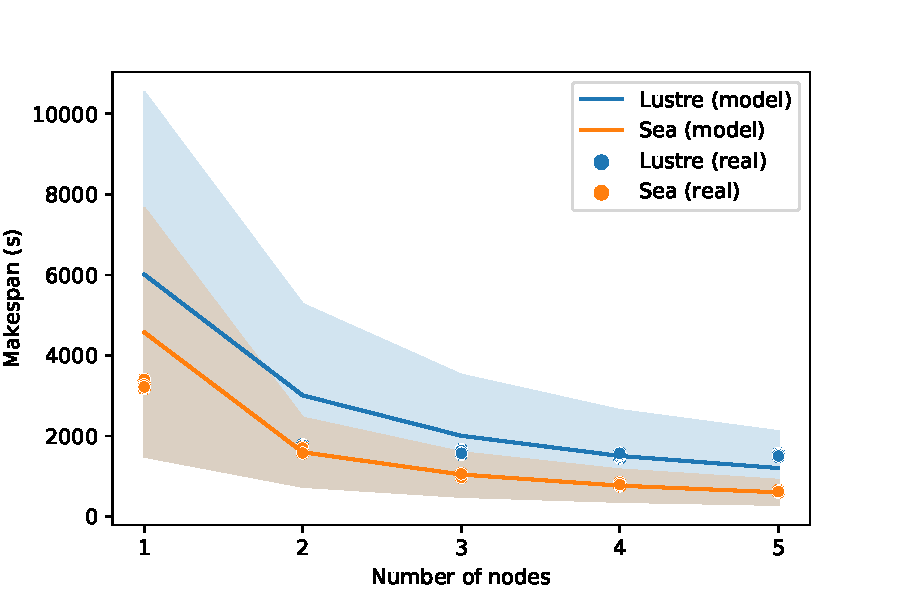
\includegraphics[width=\columnwidth]{figures/sea-comp/nodes.pdf}%
        \caption{Experiment 1: Varying the number of nodes, 10 iterations}\label{fig:sea-comp:nodes}
    \end{subfigure}
    \begin{subfigure}{0.5\columnwidth}
        \centering
        \captionsetup{width=.85\linewidth}
        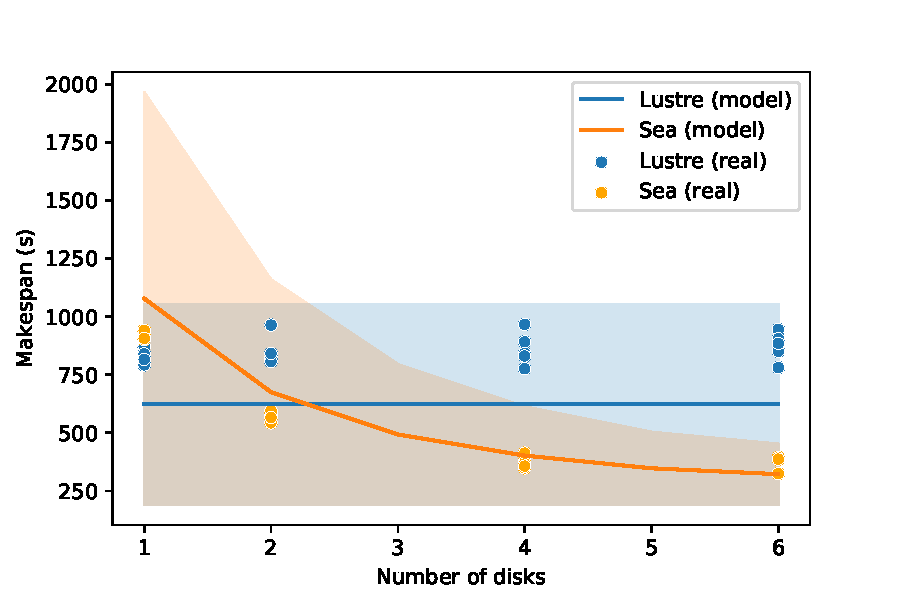
\includegraphics[width=\linewidth]{figures/sea-comp/disks.pdf}
        \caption{Experiment 2: Varying the number of disks, 5 iterations}\label{fig:sea-comp:disks}
    \end{subfigure}
    \begin{subfigure}{0.5\columnwidth}
        \centering
        \captionsetup{width=.85\linewidth}
        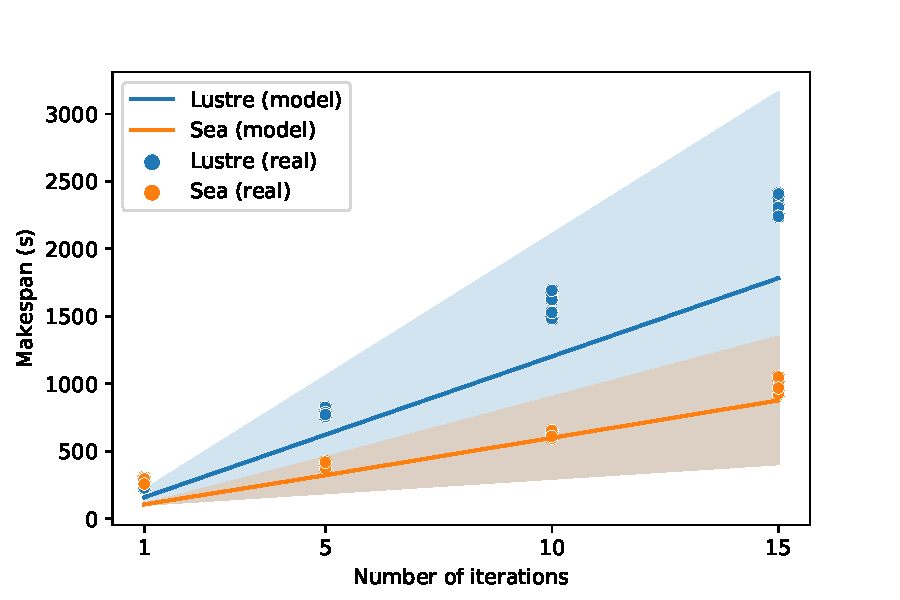
\includegraphics[width=\linewidth]{figures/sea-comp/iterations.pdf}
        \caption{Experiment 3: Varying the number of iterations}\label{fig:sea-comp:iterations}
    \end{subfigure}
    \begin{subfigure}{0.5\columnwidth}
        \centering
        \captionsetup{width=.85\linewidth}
        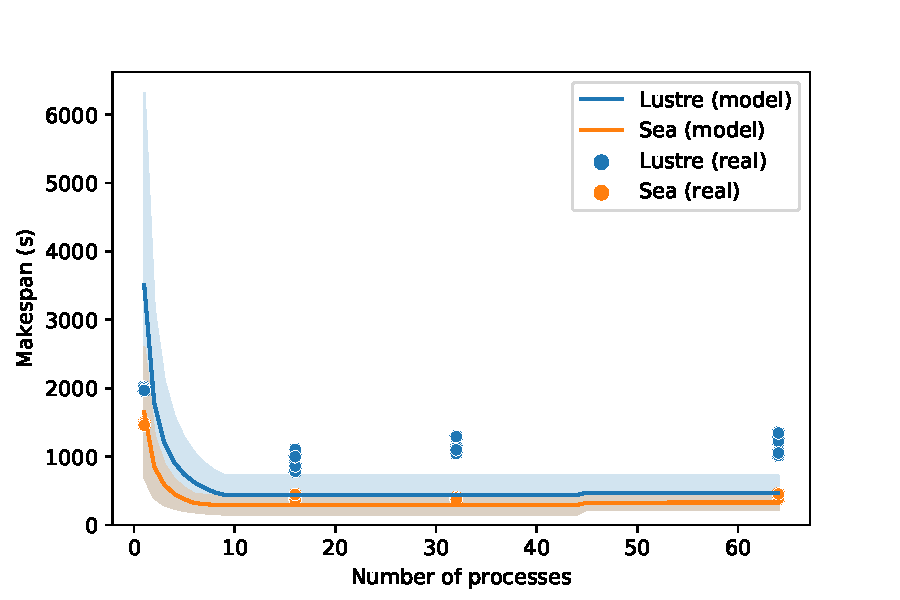
\includegraphics[width=\linewidth]{figures/sea-comp/threads.pdf}
        \caption{Experiment 4: Varying the number of parallel processes, 5 iterations}\label{fig:sea-comp:processes}
    \end{subfigure}
    \caption{Benchmarks comparing Lustre and Sea In-memory performance under various conditions using the Incrementation application
    on the Big Brain image. All experiments were repeated 5$\times$.}
    \label{fig:sea-comp:benchmarks}
    \end{figure*}

      \subsection{Sea achieves significant speedups}

      As can be seen in Figure~\ref{fig:sea-comp:benchmarks}, Sea with the
      in-memory configuration speeds up execution the majority of the
      conditions. The largest speedups observed can be seen in
      Figure~\ref{fig:sea-comp:processes} at 32 processes, where the speedup is
      nearly 3$\times$. We believe that the speedup here is primarily due to the
      contention on Lustre. While each local disk has an average of 5 processes
      trying to write concurrently to it at 32 processes, each Lustre has around
      3 concurrent processes while to it. Whereas one might assume this means
      Lustre would have less contention overall and should perform better, there
      are significant bandwidth differences to account for between the local
      disks and Lustre (see Table~\ref{table:sea-comp:fs}) that would result in
      improved local disk performance despite increased contention. Furthermore,
      Lustre has a centralized metadata server that is responsible for
      determining which OST is assigned to each block, guaranteeing a certain
      amount of load-balance on the storage disks. This is in contrast with the
      local disks, who do not rely on a metadata server and are selected by Sea
      via a random shuffling.

      The experimental conditions with the next largest speedup is in
      Figure~\ref{fig:sea-comp:iterations} at 10 iterations with a 2.6$\times$
      speedup. It is believed that Sea performs best at 10 iterations, rather
      than 15, because that is when the majority of the writes must be made to
      local disk. While Sea is not expected to surpass the Lustre makespan,
      Lustre does have a slight performance advantage in that is able to evict
      data once it is persisted to Lustre, allowing it to make more effecient
      use of memory whenever possible. 

      When varying the number of nodes (Figure~\ref{fig:sea-comp:nodes}), we
      achieved the greatest speedup at 5 nodes, with a speedup of 2.4$\times$.
      Similar to our experiments with multiprocessing, the speedup here appears
      to be due to increased contention on Lustre. However, there is one main
      difference here, and that is that only Sea is experiencing increased
      contention, as the contention within the compute nodes is fixed. Both the
      model and experimental results state that the speedup is approaching a
      plateau, however, it is expected that once the number of threads writing
      to Lustre exceeds the number of OSTs (e.g. 9 nodes), we will observe an
      even greater speedup from Sea due to the increased contention on Lustre.

      As expected, our results demonstrate that with an increase in local disk,
      we can achieve greater speedups. Our results
      (Figure~\ref{fig:sea-comp:disks}) show that at 6 disks, we achieve a
      speedup of 2$\times$. This is natural, due to the fact that the most disks
      we have, the less contention there will be on any given disk. In
      particular, in our case, each disk at 6 disks should optimally only have a
      single process writing to it.

      When Sea does not provide speedups, it either performs similarly to
      Lustre, as can be seen in Figure~\ref{fig:sea-comp:nodes} at one node and
      Figure~\ref{fig:sea-comp:iterations} at 1 iteration, or sightly slows down
      execution, as can been seen in~\ref{fig:sea-comp:disks}. As expected,
      Sea at a single iteration can at best perform similarly or slightly worse than
      Lustre. This is because all the data is read from Lustre and written to
      Lustre, operating in the same way that Lustre would with page cache.

      Sea at a single node likely performs equivalently to Lustre because
      Lustre, in this case, has very good bandwidth, having at most 6 concurrent
      writes to the whole file system. Furthermore, due to the limited number of
      concurrent writes on Lustre at any given time, Lustre needs to wait less
      for writes to flush to disk, making better use of available page cache
      space. Sea's performance, in contrast, is negatively impacted as there is
      more data being written to local storage and the combined bandwidth of the
      local storage is far less superior than that of Lustre's, due to only
      having 6 disks available.

      The contention on the disk at Sea operation with only a single local disk
      is likely the cause of the decline in performance in
      Figure~\ref{fig:sea-comp:disks}. As Lustre has significantly less
      contention on the file system, it is able to exhibit a superior
      performance to Sea. As we can see, increasing the number of local disks
      improves Sea's performance beyond what Lustre can achieve.
    

      \subsection{Model accurately predicts performance trends}

      Figure~\ref{fig:sea-comp:benchmarks} shows us that our model incorrectly predicts
      the bounds for two experiments: Experiment 3 (Figure~\ref{fig:sea-comp:iterations})
      and Experiment 4 (Figure~\ref{fig:sea-comp:processes}). In Experiment 3, the model incorrectly
      predicts the bounds for 1 iteration. Since in this case, all the data should be able to fit
      in page cache for both Sea and Lustre, it is possible that memory bandwidth has been
      overestimated, resulting in incorrect model preditions.

      We believe that Lustre exceeds the model bounds in Experiment 4 due to
      increased contention on the file system. While our model predicts that the
      disk bandwidth will be the bottleneck, thus plateauing at 9 parallel
      processes per node, there are other Lustre bottlenecks that are not
      included in the model, like the metadata server. We expect that there were
      too many incoming requests to the server at 30+ parallel processes, that
      performance declined above model bounds. 
      

    \begin{figure*}

        \centering
        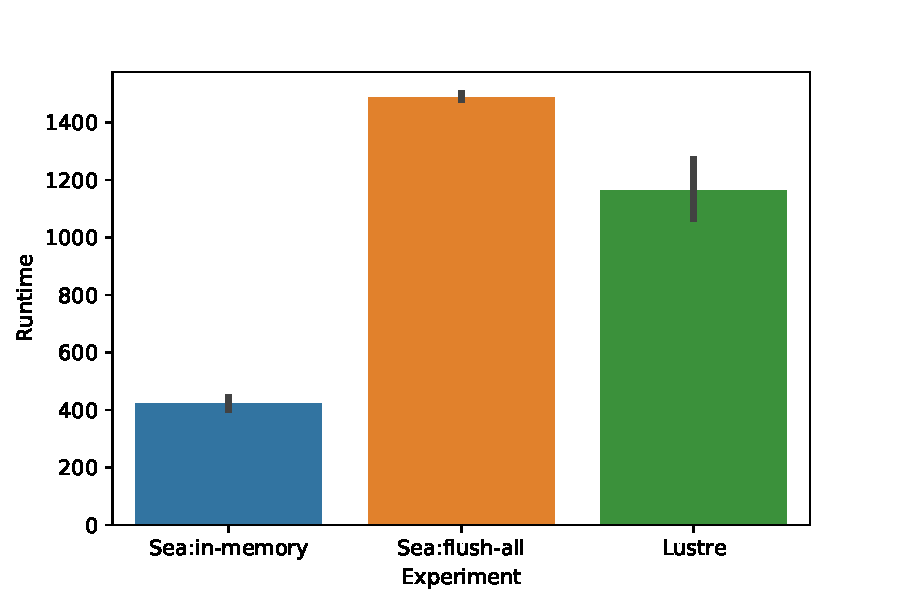
\includegraphics[width=\columnwidth]{figures/sea-comp/flushall.pdf}%
        \caption{Comparision of the different Sea modes with Lustre on the incrementation application
        processing 1000 Big Brain blocks with 5 nodes, 5 iterations, 6 disks and 6 parallel processes.}
    \label{fig:sea-comp:flush}
    \end{figure*}

      \subsection{Significant overheads with Flush-all mode on data-intensive workload}

      Figure~\ref{fig:sea-comp:flush} demonstrates the overhead that can be
      obtained by using flush-all when there is no compute to mask the flushing.
      Not only is Sea flush-all 3.5$\times$ slower than Sea in-memory, it is
      1.3$\times$ slower than Lustre. The reason for it being slower than Lustre
      is that Sea flush-all does not evict any files and had to copy files from
      local disk to Lustre, as a result. In contrast, Lustre does not make use
      of local disk space. It is able to evict data from memory once it is
      materialized to Lustre. Consequently, Lustre alone does not have the third
      overhead of writing the data to disk like Sea flush-all does. The
      performance loss is likely to not have been discernable if we had compute
      time that matched data transfer time, however, the performance gain might
      not have been as significant unless we were writing in parallel data that
      far exceeded page cache space as the application would not have to wait
      for data to be flushed to Lustre before proceeding.

\section{Discussion}

    \subsection{Lightweight data-management library for CLI applications}

    Through the interception of libc calls, Sea successfully manages to redirect
    I/O to the different available storage devices on an HPC cluster.
    Since Sea is lightweight and requires minimal configuration, it preserves
    the characteristics that are important to scientific applications.

    At minimum, Sea requires the specification of a configuration file for it to work.
    A user would need to know details on the cluster storage that can be leveraged as 
    well as approximate details on how much data an application execution can produce 
    at any given time. Due to the simplicity of the configuration file, 
    Sea maintains the ease-of-use requirement for scientific applications.

    Sea maintains whole files, as produced by the pipeline. In no instance does it modify
    or alter the data produced by the pipeline. Since there is no risk of Sea modifying
    the contents of the data, Sea preserves the reproducibility requirement.

    The flush-and-evict process may affect overall application parallelism. It
    would depend on how many Sea processes are started on the compute node. If
    only a single instance of Sea is called on a compute node, there will only
    be a single flush and evict process, and therefore, only a single flush and
    evict process will exist. However, if Sea is launched many times on a given
    node, there will be many flush and evict processes which may interfere with
    the application compute. However, our results do not indicate that
    performance is significantly impacted by the presence of a single flush and
    evict process.  

    Sea alone has limited portability. It cannot be used with operating systems that are
    not Linux-based, and therefore, the use of Sea limits application portability.
    However, HPC systems commonly use Linux operating systems, thus, it is not limiting
    for its intended use case. Furthermore, we provide publicly available containers to
    simplify the usage of Sea on various other operating systems.

    \subsection{In-memory performance with Sea}
   
    Our results indicate that Sea can significantly improve the
    performance in applications executing data-intensive workflows. In all
    experiments, we observed speedups of up to 3$\times$, with the majority of
    cases reaching a 2$\times$ speedup. In very few cases did the use of Sea not
    result in any speedups. In two of the three scenarios, Sea performed
    identically to Lustre, either because Sea was issuing the same amount of
    data transfers to Lustre or Lustre bandwidth far exceeded what was available
    locally.

    In a shared cluster environment, such as though found in high-performance
    computing clusters, it is more unlikely that the PFS would be so underused
    that it could achieve better performance than leveraging local storage, even
    if local storage was limited. We therefore believe that it is very unlikely
    obtain no speedups from using Sea on a production HPC cluster as long as the application is data intensive.
    
    For our experiments we relied on a synthetic data-intensive application,
    however, the I/O patterns exhibited by such an application do not adequately
    mimic the patterns of scientific applications. In our experiments, we
    demonstrate what the possible performance upper bound can look like and how
    it is affected by various different factors. Despite the fact that typical
    scientific workflows may not be as data-intensive, it is believed that scientific 
    applications can still benefit a significant amount by limiting writes to a shared
    PFS that is experiencing traffic generated by many other users. Furthermore,
    given that scientific applications have more compute, Sea flush-all can be used
    with reduced overheads.

    \subsection{Performance boost with local storage availability}

    As expected, Sea's performance increases with the number of disks available.
    However, our results also demonstrate that it does not require that many disks
    to surpass Lustre's performance, even when Lustre is underutilized. Therefore,
    while Sea underperformed at a single disk, it is likely that this will be sufficient
    to experience speedups even in a production environment, where Lustre has to 
    deal with user traffic across the cluster. This is important to note because it
    is not uncommon for HPC cluster compute nodes to only have a single disk available
    as burst buffer. However, should more disks be available, it would be best to include
    as many as possible in Sea.

    \subsection{Sea preferred when Lustre is overloaded}

    In instances where contention on Lustre exceeds that of local disks, Sea in-memory 
    outperforms Lustre. In all cases, it did not take very much for Sea to outperform
    Lustre. It is expected that the resource requirements of scientific applications 
    running on HPC systems could far exceed those of our current experiments, relying on
    100s of nodes instead of just 5. Therefore, data-intensive scientific applications
    would benefit greatly from using Sea.

    When Lustre is not overloaded, there is little benefit to using Sea. However, we found
    that Sea performs similarly to Lustre in these cases. Since there is no real penalty to 
    using Sea when Lustre is not overloaded, it is recommended to use Sea in all scenarios.
    Moreover, users on HPC clusters are unaware of what the PFS performance will be at the 
    time when their experiments will be scheduled. Knowing that Sea does not incur significant
    overheads will allow users to freely execute Sea without hesitation. 

    \subsection{Flush when necessary and evict often}

    The results demonstrate that flushing all of the data incurs significant
    overheads with a data-intensive application. These overheads can be so
    significant that Sea's performance, in these cases, can be found to be
    inferior to that of Lustre. In applications where data is shared or when
    results are required for post-processing, there is no other option than to
    flush this data. Since the majority of the overhead appears to have arisen
    from writing to and flushing from local disk, it is recommended that
    lesser-used data be evicted from Sea, freeing up space for newer data.

    There is limited benefit to Sea when flushing all the data in a
    data-intensive scenario. Sea must perform the same number of I/O operations
    as Lustre in these cases. While the application itself can proceed to
    completion faster, as it only needs to wait for all the data to be writted
    to local storage, the time required for the final flush of the data can be
    quite significant, particularly when flushing from disk to Lustre. Therefore,
    we recommend that flushing all the data is reserved for when applications where
    there is substantial compute time. 


    Increase in performance from eviction is not only limited to scenarios where
    all the data is flushed. Sea also benefits from eviction when using the
    in-memory option as not all data may fit in memory and thus need to be
    written to slower local storage. Sea currently cannot handle scenarios where
    the application is attempting to access a file that is in the process of being
    moved, and as a result, we were not able to use much eviction in our experiments.
    This would be an important feature to enable in future Sea releases, despite the potential
    slowdown that may be incurred from waiting for the data to be materialized to Lustre.

\section{Conclusion and future work}

    We created Sea, a lightweight open-source data-management library for
    scientific applications. With the help of libc interception, we were able to
    create a library that maintains qualities import to scientific computing
    (i.e. ease-of-use, reproducibility, portability and parallelism). Our
    results demonstrate that Sea is quite beneficial to reducing the data
    transfers overheads, particularly when using an in-memory computing
    configuration, producing speedups of up to 3$\times$. Sea's performance is,
    however, limited when the PFS is not being heavily used.

    Experimental results demonstrate that our performance model accurately
    depicts the bounds in the majority of the cases. The model overestimated
    performance when metadata calls were heavily impacting performace. This is
    because the model neglects to account for any kind of latency. More accurate
    predictions could be obtained with a more complex model, although, due to
    Lustre's complex functioning, a simulator would likely be more appropriate
    here.

    More complex functioning of Sea, such as splitting of individual files, as
    seen with the other burst buffer file systems, may be preferential,
    particularly in maximizing cache usage. However, the more we complexify
    these libraries, the harder it is for users to use. As a result, users must
    wait until the cluster guidelines are developed detailing how a user should
    use these libraries. The boundary between ease-of-use and performance needs to be
    further explored to determine what is best for users and applications.



